\chapter{Устойчивость}
\label{ch:2}

Отличительной особенностью функциональных структур данных является то,
что они всегда \term{устойчивы}{persistent}~--- обновление
функциональной структуры не уничтожает старую версию, а создает
новую, которая с ней сосуществует. Устойчивость достигается путем
\emph{копирования} затронутых узлов структуры данных, и все изменения
проводятся на копии, а не на оригинале. Поскольку узлы никогда
напрямую не модифицируются, все незатронутые узлы могут
\term{совместно использоваться}{be shared} между старой и новой версией структуры
данных без опасения, что изменения одной версии непроизвольно окажутся
видны другой.

В этой главе мы исследуем подробности копирования и совместного использования для
двух простых структур данных: списков и двоичных деревьев.

\section{Списки}
\label{sc:2.1}

Мы начинаем с простых связанных списков, часто встречающихся в
императивном программировании и вездесущих в функциональном.  Основные
функции, поддерживаемые списками, в сущности те же, что и для
абстракции стека, описанной в виде сигнатуры на Стандартном ML на
Рис.~\ref{fig:2.1}.  Списки и стеки можно тривиально реализовать либо
с помощью встроенного типа <<список>> (Рис.~\ref{fig:2.2}), либо как
отдельный тип (Рис.~\ref{fig:2.3}).

\begin{remark}
Сигнатура на Рис.~\ref{fig:2.1} использует терминологию списков
(\texttt{cons}, \texttt{head}, \texttt{tail}), а не стеков
(\texttt{push}, \texttt{top}, \texttt{pop}), потому что мы
рассматриваем списки как частный случай общего класса
последовательностей. Другими примерами этого класса являются
\emph{очереди}, \emph{двусторонние очереди} и \emph{списки с
  конкатенацией}. Для функций во всех этих абстракциях мы используем
одинаковые соглашения по именованию, чтобы можно было заменять одну
реализацию другой с минимальными трудностями.
\end{remark}

\begin{figure}
\begin{lstlisting}
signature Stack = sig
  type $\alpha$ Stack
  val empty   : $\alpha$ Stack
  val isEmpty : $\alpha$ Stack $\rightarrow$ bool
  val cons    : $\alpha \times \alpha$ Stack $\rightarrow$ $\alpha$ Stack
  val head    : $\alpha$ Stack $\rightarrow \alpha$ Stack /*$\mbox{ возбуждает EMPTY для пустого стека }$*/
  val tail    : $\alpha$ Stack $\rightarrow \alpha$ Stack /*$\mbox{ возбуждает EMPTY для пустого стека }$*/
end
\end{lstlisting}
% TODO: Эта херня пихает курсив, когда у меня камлёвые комментарии. Разобраться.
% \centering

\caption{Сигнатура для стеков.}  \label{fig:2.1}
\end{figure}


\begin{figure}
\begin{lstlisting}
structure List : Stack = structure
  type $\alpha$ Stack =  $\alpha$ list
  val empty = []
  fun isEmpty s = null s
  fun cons (x,s) = x::s
  fun head s     = hd s
  fun tail s     = tl s
end
\end{lstlisting}
\caption{Реализация стека с помощью встроенного типа списков.}\label{fig:2.2}
\end{figure}

\begin{figure}
\begin{lstlisting}
structure CustomStack: Stack = structure
  datatype $\alpha$ Stack = Nil | Cons of $\alpha \times \alpha$ Stack
  val empty = Nil
  fun isEmpty Nil = true | isEmpty _ = false
  fun cons (x,s) = Cons (x, s)
  fun head Nil   = raise EMPTY
    | head (Cons(x,s)) = x

  fun tail Nil   = raise EMPTY
    | tail (Cons(x,s)) = s
end
\end{lstlisting}
  \caption{Реализация стека в виде отдельного типа.}
  \label{fig:2.3}
\end{figure}

К этой сигнатуре мы могли бы добавить ещё одну часто встречающуюся
операцию на списках: $\concat$, которая конкатенирует (т. е.,
соединяет) два списка. В императивной среде эту функцию нетрудно
поддержать за время $O(1)$, если сохранять указатели и на первый, и на
последний элемент списка.  Тогда $\concat$ просто изменяет последнюю
ячейку первого списка так, чтобы она указывала на первую ячейку
второго списка.  Результат этой операции графически показан на
Рис.~\ref{fig:2.4}. Обратите внимание, что эта операция
\emph{уничтожает} оба своих аргумента~--- после выполнения
\lstinline!xs $\concat$ ys! ни \lstinline!xs!, ни \lstinline!ys! использовать
больше нельзя.

\begin{figure}[h]
  \centering
	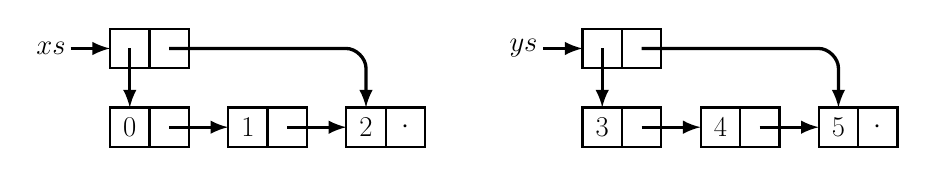
\begin{tikzpicture}[thick,scale=0.5, every node/.style={scale=0.5}]
    \tikzstyle{marrs}=[very thick,-latex]

    \begin{scope}
    
        \foreach \x/\y in {0/0, 0/-2, 3/-2, 6/-2} {
            \draw (\x - 0.5, \y - 0.5) rectangle +(1, 1); \draw (\x + 1 - 0.5, \y - 0.5) rectangle +(1, 1);
        }
        \draw[marrs] (-1.5, 0) -> +(1, 0);
        \draw[marrs] (0, 0) -> +(0, -1.5);
        \draw[marrs] (1, -2) -> +(1.5, 0);
        \draw[marrs] (4, -2) -> +(1.5, 0);
        \draw[marrs] (1, 0) -- (5.5, 0) .. controls (5.75, 0) and (6, -0.25) .. (6, -0.5) -- (6, -1.5);
        
        { \huge
            \draw (-2, 0) node {$xs$};
            \draw (0, -2) node {$0$};
            \draw (3, -2) node {$1$};
            \draw (6, -2) node {$2$};
            \draw (7, -2) node {$\cdot$};
        }
    
    \end{scope}
    
    \begin{scope}[xshift=12cm]
    
        \foreach \x/\y in {0/0, 0/-2, 3/-2, 6/-2} {
            \draw (\x - 0.5, \y - 0.5) rectangle +(1, 1); \draw (\x + 1 - 0.5, \y - 0.5) rectangle +(1, 1);
        }
        \draw[marrs] (-1.5, 0) -> +(1, 0);
        \draw[marrs] (0, 0) -> +(0, -1.5);
        \draw[marrs] (1, -2) -> +(1.5, 0);
        \draw[marrs] (4, -2) -> +(1.5, 0);
        \draw[marrs] (1, 0) -- (5.5, 0) .. controls (5.75, 0) and (6, -0.25) .. (6, -0.5) -- (6, -1.5);
        
        { \huge
            \draw (-2, 0) node {$ys$};
            \draw (0, -2) node {$3$};
            \draw (3, -2) node {$4$};
            \draw (6, -2) node {$5$};
            \draw (7, -2) node {$\cdot$};
        }
    \end{scope}
    
    
    
\end{tikzpicture}\par
  (до)\par
	\vspace{0.5cm}
	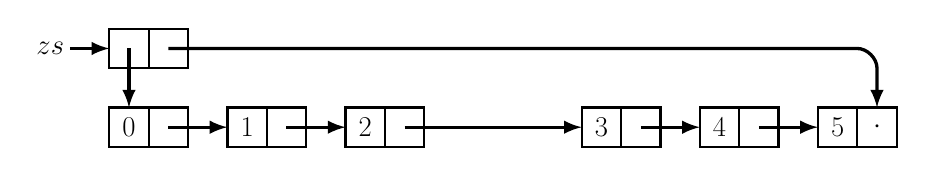
\begin{tikzpicture}[thick,scale=0.5, every node/.style={scale=0.5}]
    \tikzstyle{marrs}=[very thick,-latex]

    
    \begin{scope}
    
        \foreach \x/\y in {0/0, 0/-2, 3/-2, 6/-2} {
            \draw (\x - 0.5, \y - 0.5) rectangle +(1, 1); \draw (\x + 1 - 0.5, \y - 0.5) rectangle +(1, 1);
        }
        \draw[marrs] (-1.5, 0) -> +(1, 0);
        \draw[marrs] (0, 0) -> +(0, -1.5);
        \draw[marrs] (1, -2) -> +(1.5, 0);
        \draw[marrs] (4, -2) -> +(1.5, 0);
        \draw[marrs] (1, 0) -- (18.5, 0) .. controls (18.75, 0) and (19, -0.25) .. (19, -0.5) -- (19, -1.5);
        \draw[marrs] (7, -2) -- +(4.5, 0);
        
        { \huge
            \draw (-2, 0) node {$zs$};
            \draw (0, -2) node {$0$};
            \draw (3, -2) node {$1$};
            \draw (6, -2) node {$2$};
        }
    
    \end{scope}
    
    \begin{scope}[xshift=12cm]
    
        \foreach \x/\y in {0/-2, 3/-2, 6/-2} {
            \draw (\x - 0.5, \y - 0.5) rectangle +(1, 1); \draw (\x + 1 - 0.5, \y - 0.5) rectangle +(1, 1);
        }
        
        \draw[marrs] (1, -2) -> +(1.5, 0);
        \draw[marrs] (4, -2) -> +(1.5, 0);
        
        { \huge
            \draw (0, -2) node {$3$};
            \draw (3, -2) node {$4$};
            \draw (6, -2) node {$5$};
            \draw (7, -2) node {$\cdot$};
        }
    \end{scope}
    
    
    
\end{tikzpicture}\par
  (после)\par
	\vspace{0.5cm}
  \caption{Выполнение \lstinline!xs $\concat$ ys! в императивной среде. Эта операция уничтожает списки-аргументы \lstinline!xs! и \lstinline!ys!.}
  \label{fig:2.4}
\end{figure}

В функциональном окружении мы не можем деструктивно модифицировать
последнюю ячейку первого списка. Вместо этого мы копируем эту ячейку и
модифицируем хвостовой указатель в ячейке-копии. Затем мы копируем
предпоследнюю ячейку и модифицируем ее хвостовой указатель, указывая
на копию последней ячейки.  Такое копирование продолжается, пока
не окажется скопирован  весь список. Процесс в общем виде можно
реализовать как
\begin{lstlisting}
  fun xs$\concat$ys = if isEmpty xs then ys else cons (head xs, tail xs$\concat$ys)
\end{lstlisting}
Если у нас есть доступ к реализации нашей структуры (например, в виде
встроенных списков Стандартного ML), мы можем переписать эту функцию
через сопоставление с образцом:
\begin{lstlisting}
  fun []$\concat$ys = ys
    | (x :: xs)$\concat$ys = x :: (xs$\concat$ys)
\end{lstlisting}
На Рис.~\ref{fig:2.5} изображен результат конкатенации двух
списков. Обратите внимание, что после выполнения операции мы можем
продолжать использовать два исходных списка, \lstinline!xs! и
\lstinline!ys!. Таким образом, мы добиваемся устойчивости, но за счет
копирования ценой $O(n)$.\footnote{%
  В Главах~\ref{ch:10} и \ref{ch:11} мы увидим, как можно поддержать
  $\concat$ за время $O(1)$ без потери устойчивости.
}

\begin{figure}[h]
  \centering
	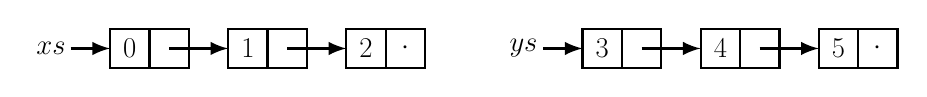
\begin{tikzpicture}[thick,scale=0.5, every node/.style={scale=0.5}]
    \tikzstyle{marrs}=[very thick,-latex]

    \begin{scope}
    
        \foreach \x/\y in {0/0, 3/0, 6/0} {
            \draw (\x - 0.5, \y - 0.5) rectangle +(1, 1); \draw (\x + 1 - 0.5, \y - 0.5) rectangle +(1, 1);
        }
        \draw[marrs] (-1.5, 0) -> +(1, 0);
        \draw[marrs] (1, 0) -> +(1.5, 0);
        \draw[marrs] (4, 0) -> +(1.5, 0);
        
        { \huge
            \draw (-2, 0) node {$xs$};
            \draw (0, 0) node {$0$};
            \draw (3, 0) node {$1$};
            \draw (6, 0) node {$2$};
            \draw (7, 0) node {$\cdot$};
        }
    
    \end{scope}
    
    \begin{scope}[xshift=12cm]
    
        \foreach \x/\y in {0/0, 3/0, 6/0} {
            \draw (\x - 0.5, \y - 0.5) rectangle +(1, 1); \draw (\x + 1 - 0.5, \y - 0.5) rectangle +(1, 1);
        }
        \draw[marrs] (-1.5, 0) -> +(1, 0);
        \draw[marrs] (1, 0) -> +(1.5, 0);
        \draw[marrs] (4, 0) -> +(1.5, 0);
        
        { \huge
            \draw (-2, 0) node {$ys$};
            \draw (0, 0) node {$3$};
            \draw (3, 0) node {$4$};
            \draw (6, 0) node {$5$};
            \draw (7, 0) node {$\cdot$};
        }
    \end{scope}
    
    
    
\end{tikzpicture}\par
  (до)\par
	\vspace{0.5cm}
	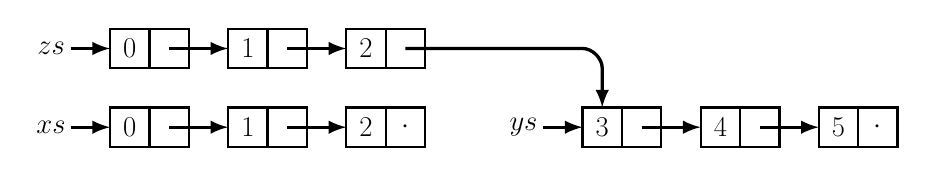
\begin{tikzpicture}[thick,scale=0.5, every node/.style={scale=0.5}]
    \tikzstyle{marrs}=[very thick,-latex]
    
    
    
    \begin{scope}
    
        \foreach \x/\y in {0/0, 3/0, 6/0} {
            \draw (\x - 0.5, \y - 0.5) rectangle +(1, 1); \draw (\x + 1 - 0.5, \y - 0.5) rectangle +(1, 1);
        }
        \draw[marrs] (-1.5, 0) -> +(1, 0);
        \draw[marrs] (1, 0) -> +(1.5, 0);
        \draw[marrs] (4, 0) -> +(1.5, 0);
        
        { \huge
            \draw (-2, 0) node {$xs$};
            \draw (0, 0) node {$0$};
            \draw (3, 0) node {$1$};
            \draw (6, 0) node {$2$};
            \draw (7, 0) node {$\cdot$};
        }
    
    \end{scope}
    
    \begin{scope}[xshift=12cm]
    
        \foreach \x/\y in {0/0, 3/0, 6/0} {
            \draw (\x - 0.5, \y - 0.5) rectangle +(1, 1); \draw (\x + 1 - 0.5, \y - 0.5) rectangle +(1, 1);
        }
        \draw[marrs] (-1.5, 0) -> +(1, 0);
        \draw[marrs] (1, 0) -> +(1.5, 0);
        \draw[marrs] (4, 0) -> +(1.5, 0);
        
        { \huge
            \draw (-2, 0) node {$ys$};
            \draw (0, 0) node {$3$};
            \draw (3, 0) node {$4$};
            \draw (6, 0) node {$5$};
            \draw (7, 0) node {$\cdot$};
        }
    \end{scope}
    
    \begin{scope}[yshift=2cm]
    
        \foreach \x/\y in {0/0, 3/0, 6/0} {
            \draw (\x - 0.5, \y - 0.5) rectangle +(1, 1); \draw (\x + 1 - 0.5, \y - 0.5) rectangle +(1, 1);
        }
        \draw[marrs] (-1.5, 0) -> +(1, 0);
        \draw[marrs] (1, 0) -> +(1.5, 0);
        \draw[marrs] (4, 0) -> +(1.5, 0);
        
        { \huge
            \draw (-2, 0) node {$zs$};
            \draw (0, 0) node {$0$};
            \draw (3, 0) node {$1$};
            \draw (6, 0) node {$2$};
            
            \draw[marrs] (7, 0) -- (11.5, 0) .. controls (11.75, 0) and (12, -0.25) .. (12, -0.5) -- (12, -1.5);
        }
    
    \end{scope}
    
    
    
\end{tikzpicture}\par
  (после)\par
	\vspace{0.5cm}
  \caption{Выполнение \lstinline!zs = xs$\concat$ys! в функциональной среде. Заметим, что списки-аргументы \lstinline!xs! и \lstinline!ys! не затронуты операцией.}
  \label{fig:2.5}
\end{figure}

Несмотря на большой объем копирования, заметим, что второй список, \lstinline!ys!, нам
копировать не пришлось. Эти узлы теперь общие между
\lstinline!ys! и \lstinline!zs!. Ещё одна функция, иллюстрирующая
парные понятия копирования и общности подструктур~---
\lstinline!update!, изменяющая значение узла списка по данному
индексу. Эту функцию можно реализовать как
\begin{lstlisting}
  fun update ([], i, y) = raise Subscript
    | update (x::xs, 0, y) = y::xs
    | update (x::xs, i, y) = x::update(xs, i-1, y)
\end{lstlisting}
Здесь мы не копируем весь список-аргумент. Копировать приходится
только сам узел, подлежащий модификации (узел $i$) и узлы,
содержащие прямые или косвенные указатели на $i$.  Другими словами,
чтобы изменить один узел, мы копируем все узлы на пути от корня
к изменяемому. Все узлы, не находящиеся на этом пути, используются как
исходной, так и обновленной версиями. На Рис.~\ref{fig:2.6} показан
результат изменения третьего узла в пятиэлементном списке: первые
три узла копируются, а последние два используются совместно.

\begin{figure}[h]
  \centering
	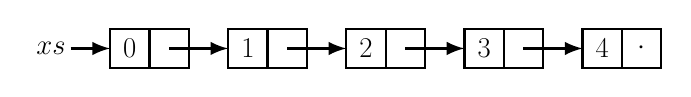
\begin{tikzpicture}[thick,scale=0.5, every node/.style={scale=0.5}]
    \tikzstyle{marrs}=[very thick,-latex]

    \begin{scope}
    
        \foreach \x/\y in {0/0, 3/0, 6/0, 9/0, 12/0} {
            \draw (\x - 0.5, \y - 0.5) rectangle +(1, 1); \draw (\x + 1 - 0.5, \y - 0.5) rectangle +(1, 1);
        }
        \draw[marrs] (-1.5, 0) -> +(1, 0);
        \foreach \x in {1, 4, 7, 10} {
            \draw[marrs] (\x, 0) -> +(1.5, 0);
        }
        
        { \huge
            \draw (-2, 0) node {$xs$};
            \foreach \x/\y in {0/0, 3/1, 6/2, 9/3, 12/4} {
                \draw (\x, 0) node {$\y$};
            }
            \draw (13, 0) node {$\cdot$};
        }
    
    \end{scope}
    
\end{tikzpicture}\par
  (до)\par
	\vspace{0.5cm}
	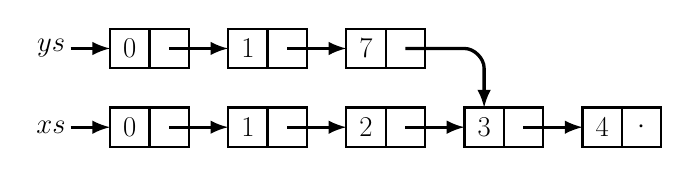
\begin{tikzpicture}[thick,scale=0.5, every node/.style={scale=0.5}]
    \tikzstyle{marrs}=[very thick,-latex]
    
    
    
    \begin{scope}
    
        \foreach \x/\y in {0/0, 3/0, 6/0, 9/0, 12/0} {
            \draw (\x - 0.5, \y - 0.5) rectangle +(1, 1); \draw (\x + 1 - 0.5, \y - 0.5) rectangle +(1, 1);
        }
        \draw[marrs] (-1.5, 0) -> +(1, 0);
        \foreach \x in {1, 4, 7, 10} {
            \draw[marrs] (\x, 0) -> +(1.5, 0);
        }
        
        { \huge
            \draw (-2, 0) node {$xs$};
            \foreach \x/\y in {0/0, 3/1, 6/2, 9/3, 12/4} {
                \draw (\x, 0) node {$\y$};
            }
            \draw (13, 0) node {$\cdot$};
        }   
    
    \end{scope}
    
    \begin{scope}[yshift=2cm]
    
        \foreach \x/\y in {0/0, 3/0, 6/0} {
            \draw (\x - 0.5, \y - 0.5) rectangle +(1, 1); \draw (\x + 1 - 0.5, \y - 0.5) rectangle +(1, 1);
        }
        \draw[marrs] (-1.5, 0) -> +(1, 0);
        \draw[marrs] (1, 0) -> +(1.5, 0);
        \draw[marrs] (4, 0) -> +(1.5, 0);
        
        { \huge
            \draw (-2, 0) node {$ys$};
            \draw (0, 0) node {$0$};
            \draw (3, 0) node {$1$};
            \draw (6, 0) node {$7$};
            
            \draw[marrs] (7, 0) -- (8.5, 0) .. controls (8.75, 0) and (9, -0.25) .. (9, -0.5) -- (9, -1.5);
        }
    
    \end{scope}
    
    
    
\end{tikzpicture}\par
  (после)\par
	\vspace{0.5cm}

  \caption{Выполнение \lstinline!ys = update(xs, 2, 7)!. Обратите
    внимание на совместное использование структуры списками \lstinline!xs! и \lstinline!ys!.}
  \label{fig:2.6}
\end{figure}

\begin{remark}
  Такой стиль программирования очень сильно упрощается при наличии
  автоматической сборки мусора. Очень важно освободить память от тех
  копий, которые больше не нужны, но многочисленные совместно используемые
  узлы делают ручную сборку мусора нетривиальной задачей.
\end{remark}

\begin{exercise}\label{ex:2.1}
  Напишите функцию \lstinline!suffixes! типа
  \lstinline!$\alpha$ list $\to$ $\alpha$ list list!, которая принимает как
  аргумент список \lstinline!xs! и возвращает список всех его
  суффиксов в убывающем порядке длины. Например,
  \begin{lstlisting}
    suffixes [1,2,3,4] = [[1,2,3,4],[2,3,4],[3,4],[4],[]]
  \end{lstlisting}
  Покажите, что список суффиксов можно породить за время $O(n)$ и
  занять при этом $O(n)$ памяти.
\end{exercise}

\section{Двоичные деревья поиска}
\label{sc:2.2}

Если узел структуры содержит более одного указателя, оказываются
возможны более сложные сценарии совместного использования памяти. Хорошим примером
совместного использования такого вида служат двоичные деревья поиска.

Двоичные деревья поиска~--- это двоичные деревья, в которых элементы
хранятся во внутренних узлах в \term{симметричном}{symmetric}
порядке, то есть, элемент в каждом узле больше любого элемента в
левом поддереве этого узла и меньше любого элемента в правом
поддереве. В Стандартном ML мы представляем двоичные деревья поиска
при помощи следующего типа:
\begin{lstlisting}
  datatype Tree = E | T of Tree $\times$ Elem $\times$ Tree
\end{lstlisting}
где \lstinline!Elem!~--- какой-либо фиксированный полностью упорядоченный
тип элементов.

\begin{remark}
  Двоичные деревья поиска не являются полиморфными относительно типа
  элементов, поскольку в качестве элементов не может выступать любой
  тип~--- подходят только типы, снабженные отношением полного
  порядка. Однако это не значит, что для каждого типа элементов мы
  должны заново реализовывать деревья двоичного поиска. Вместо этого
  мы делаем тип элементов и прилагающиеся к нему функции сравнения
  параметрами \term{функтора}{functor}, реализующего двоичные деревья
  поиска (см. Рис.~\ref{fig:2.9}).
\end{remark}

Мы используем это представление для реализации множеств. Однако оно
легко адаптируется и для других абстракций (например, конечных
отображений) или поддержки более изысканных функций (скажем, найти
$i$-й по порядку элемент), если добавить в конструктор \lstinline!T!
дополнительные поля.

На Рис.~\ref{fig:2.7} показана минимальная сигнатура для множеств. Она
содержит значение <<пустое множество>>, а также функции добавления
нового элемента и проверки на членство.  В более практической
реализации, вероятно, будут присутствовать и многие другие функции,
например, для удаления элемента или перечисления всех элементов.

\begin{figure}
\begin{lstlisting}
signature SET = sig
  type Elem
  type Set
  val empty : Set
  val insert : Elem $\times$ Set -> Set
  val member : Elem $\times$ Set -> bool
end
\end{lstlisting}
  \caption{Сигнатура для множеств.}
  \label{fig:2.7}
\end{figure}

Функция \lstinline!member! ищет в дереве, сравнивая запрошенный
элемент с находящимся в корне дерева. Если запрошенный элемент меньше
корневого, мы рекурсивно ищем в левом поддереве. Если он больше,
рекурсивно ищем в правом поддереве. Наконец, в оставшемся случае
запрошенный элемент равен корневому, и мы возвращаем значение
<<истина>>. Если мы когда-либо натыкаемся на пустое дерево, значит,
запрашиваемый элемент не является членом множества, и мы возвращаем
значение <<ложь>>.  Эта стратегия реализуется так:
\begin{lstlisting}
  fun member(x,E) = false
    | member(x,T(a,y,b)) =
       if x < y then member(x,a)
       else if x > y then member(x,b)
       else true
\end{lstlisting}
\begin{remark}
  Простоты ради, мы предполагаем, что функции сравнения называются $<$
  и $>$. Однако если эти функции передаются в качестве параметров
  функтора, как на Рис.~\ref{fig:2.9}, часто оказывается удобнее
  называть их именами вроде \lstinline!lt! или \lstinline!leq!, а
  символы $<$ и $>$ оставить для сравнения целых и других элементарных
  типов.
\end{remark}

Функция \lstinline!insert! проводит поиск в дереве по той же стратегии,
что и \lstinline!member!, но только по пути она копирует каждый
элемент. Когда наконец оказывается достигнут пустой узел, он
заменяется на узел, содержащий новый элемент.
\begin{lstlisting}
  fun insert(x,E) = T(E,x,E)
    | insert(x, s as T(a,y,b)) =
       if x < y then T(insert(x,a),y,b)
       else if x > y then T(a,y,insert(x,b))
       else s
\end{lstlisting}
На Рис.~\ref{fig:2.8} показана типичная вставка. Каждый скопированный
узел использует одно из поддеревьев совместно с исходным деревом; речь о том поддереве,
которое не оказалось на пути поиска. Для большинства деревьев путь
поиска содержит лишь небольшую долю узлов в дереве. Громадное
большинство узлов находятся в совместно используемых поддеревьях.

\begin{figure}[h]
  \centering
	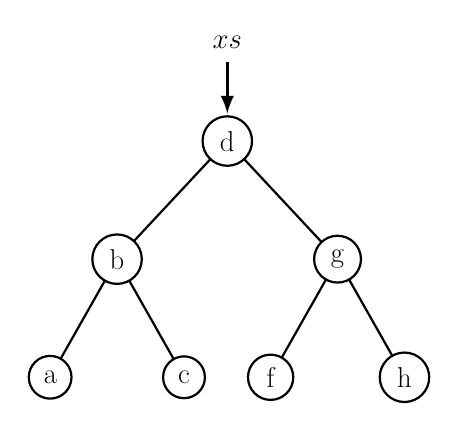
\begin{tikzpicture}[thick,scale=0.5, every node/.style={scale=0.5},level distance=3cm]
    \tikzstyle{marrs}=[very thick,-latex]
    \tikzstyle{tnode}=[circle, draw=black,node distance=1.7cm]
    \tikzstyle{level 1}=[sibling distance=5.6cm]
    \tikzstyle{level 2}=[sibling distance=3.4cm]


    \huge

    \draw (0, 2.5) node {$xs$};
    \draw[marrs] (0, 2) -- (0, 0.7);
    \node[tnode] {d}
    child {node[tnode] {b}
        child {node[tnode] {a}}
        child {node[tnode] {c}}
    }
    child {node[tnode] {g}
        child {node[tnode] {f}}
        child {node[tnode] {h}}
    };
    
\end{tikzpicture}\par
  (до)\par
	\vspace{0.5cm}
	\begin{tikzpicture}[thick,scale=0.5, every node/.style={scale=0.5},level distance=3cm]
    \tikzstyle{marrs}=[very thick,-latex]
    \tikzstyle{tnode}=[circle, draw=black,node distance=1.7cm]
    \tikzstyle{level 1}=[sibling distance=5.6cm]
    \tikzstyle{level 2}=[sibling distance=3.4cm]
    
    \huge

    \draw (0, 2.5) node {$xs$};
    \draw[marrs] (0, 2) -- +(0, -1.3);
    
    \draw (1.7, 2.5) node {$ys$};
    \draw[marrs] (1.7, 2) -- +(0, -1.3);
    
    \node[tnode] (n_d) {d}
    child {node[tnode] (n_b) {b}
        child {node[tnode] (n_a) {a}}
        child {node[tnode] (n_c) {c}}
    }
    child {node[tnode] (n_g) {g}
        child {node[tnode] (n_f) {f}
        node[tnode] (n_f') [right of=n_f] {f} [clockwise from=250]
        child {node[tnode] (n_e) {e}}
        }
        child {node[tnode] (n_h) {h}}
        node[tnode] (n_g') [right of=n_g] {g}
    }
    node[tnode] (n_d') [right of=n_d]{d};
    
    \path (n_d') edge (n_b);
    \path (n_d') edge (n_g');
    \path (n_g') edge (n_f');
    \path (n_g') edge (n_h);
    
\end{tikzpicture}\par
  (после)\par
	\vspace{0.5cm}
  \caption{Выполнение \lstinline!ys = insert("e", xs)!. Как и прежде,
    обратите внимание на совместное использвание структуры деревьями \lstinline!xs! и \lstinline!ys!.}
  \label{fig:2.8}
\end{figure}

На Рис.~\ref{fig:2.9} показано, как двоичные деревья поиска можно
реализовать в виде функтора на Стандартном ML. Функтор принимает тип
элементов и связанные с ним функции сравнения как параметры. Поскольку
часто те же самые параметры будут использоваться и другими функторами
(см., например, Упражнение~\ref{ex:2.6}), мы упаковываем их в
структуру с сигнатурой \lstinline!Ordered!.

\begin{figure}
\begin{lstlisting}
signature ORDERED = sig
  /*$\mbox{ Полностью упорядоченный тип и его функции сравнения }$*/
  type T
  val eq  : T $\times$ T -> bool
  val lt  : T $\times$ T -> bool
  val leq : T $\times$ T -> bool
end

functor UnbalancedSet(Element: ORDERED): SET = struct
  type Elem = Element.T
  datatype Tree = E | T of Tree $\times$ Elem $\times$ Tree
  type Set = Tree

  val empty = E
  fun member (x,E) = false
    | member (x,T(a,y,b)) =
       if Element.lt (x,y) then member (x,a)
       else Element.lt (y,x) then member (x,b)
       else true

  fun insert (x,E) = T(E,x,E)
    | insert (x,s as T(a,y,b)) =
       if Element.lt (x,y) then T(insert (x,a),y,b)
       else Element.lt (y,x) then T(a,y,insert (x,b))
       else s
end
\end{lstlisting}
  \caption{Реализация двоичных деревьев поиска в виде функтора на Стандартном ML.}
  \label{fig:2.9}
\end{figure}

\begin{exercise}\textbf{Андерсон \cite{Andersson1991}}\label{ex:2.2}
В худшем случае \lstinline!member! производит $2d$ сравнений, где
$d$~--- глубина дерева. Перепишите ее так, чтобы она делала не более
$d+1$ сравнений, сохраняя элемент, который \emph{может} оказаться
равным запрашиваемому (например, последний элемент, для которого
операция $<$ вернула значение <<истина>> или $\le$~--- <<ложь>>, и
производя проверку на равенство только по достижении дна дерева.
\end{exercise}

\begin{exercise}\label{ex:2.3}
  Вставка уже существующего элемента в двоичное дерево поиска копирует
  весь путь поиска, хотя скопированные узлы неотличимы от
  исходных. Перепишите \lstinline!insert! так, чтобы она избегала
  копирования с помощью исключений. Установите только один обработчик
  исключений для всей операции поиска, а не по обработчику на итерацию.
\end{exercise}

\begin{exercise}\label{ex:2.4}
  Совместите улучшения из предыдущих двух упражнений, и получите
  версию \lstinline!insert!, которая не делает ненужного копирования и
  использует не более $d+1$ сравнений.
\end{exercise}

\begin{exercise}\label{ex:2.5}
  Совместное использование может быть полезно и внутри одного объекта, не
  обязательно между двумя различными.  Например, если два поддерева
  одного дерева идентичны, их можно представить одним и тем же
  деревом.
  \begin{enumerate}
  \item Используя эту идею, напишите функцию \lstinline!complete! типа
    \lstinline!Elem $\times$ Int $\to$ Tree!, такую, что
    \lstinline!complete(x,d)! создает полное двоичное дерево глубины
    \lstinline!d!, где в каждом узле содержится \lstinline!x!.
    (Разумеется, такая функция бессмысленна для абстракции множества,
    но она может оказаться полезной для какой-либо другой абстракции,
    например, мультимножества.) Функция должна работать за время $O(d)$.
  \item Расширьте свою функцию, чтобы она строила сбалансированные
    деревья произвольного размера. Эти деревья не всегда будут полны,
    но они должны быть как можно более сбалансированными: для любого
    узла размеры поддеревьев должны различаться не более чем на
    единицу. Функция должна работать за время $O(\log n)$. (Подсказка:
    воспользуйтесь вспомогательной функцией \lstinline!create2!,
    которая, получая размер $m$, создает пару деревьев~--- одно размера
    $m$, а другое размера $m+1$)
  \end{enumerate}
\end{exercise}

\begin{exercise}\label{ex:2.6}
  Измените функтор \lstinline!UnbalancedSet! так, чтобы он служил
  реализацией не множеств, а \term{конечных отображений}{finite maps}. На
  Рис.~\ref{fig:2.10} приведена минимальная сигнатура для конечных
  отображений. (Заметим, что исключение \lstinline!NotFound! не
  является встроенным в Стандартный ML~--- Вам придется его определить
  самостоятельно. Это исключение можно было бы сделать частью
  сигнатуры \lstinline!FiniteMap!,  чтобы каждая реализация
  определяла собственное исключение \lstinline!NotFound!, но удобнее,
  если все конечные отображения будут использовать одно и то же
  исключение.)
\end{exercise}

\begin{figure}
\begin{lstlisting}
signature FINITEMAP = sig
  type Key
  type $\alpha$ Map
  val empty : $\alpha$ Map
  val bind  : Key $\times$ $\alpha$ $\times$ $\alpha$ Map $\rightarrow \alpha$ Map
  val lookup: Key $\times$ $\alpha$ Map $\rightarrow \alpha$ /*$\mbox{ возбуждает NOTFOUND, если ключ не найден }$*/
end
\end{lstlisting}
  \caption{Сигнатура для конечных отображений.}
  \label{fig:2.10}
\end{figure}

\section{Примечания}
\label{sc:2.3}

Майерс \cite{Myers1982,Myers1984} использовал копирование и совместное использование
при реализации двоичных деревьев поиска (в его случае это были
AVL-деревья).  Для общего метода реализации устойчивых структур данных
путем копирования затронутых узлов
Сарнак и Тарьян \cite{SarnakTarjan1986a} выбрали термин
\term{копирование путей}{path copying}. Существуют также другие методы
реализации устойчивых структур данных, предложенные Дрисколлом,
Сарнаком, Слейтором и Тарьяном \cite{Driscoll-etal1989} и Дитцем
\cite{Dietz1989}, но эти методы не являются чисто функциональными.

%%% Local Variables:
%%% mode: latex
%%% TeX-master: "pfds"
%%% End:
